\chapter{Vorgehen}
\label{chap:vorgehen}

% Dieses Kapitel beschreibt das methodische Vorgehen, welches in der Arbeit angewendet wurde. Erwähnen Sie hier die verschiedenen Phasen der Arbeit und ihre Ergebnisse. Arbeiten mit hohem Softwareentwicklungs-Anteil lehnen sich am besten an eine etablierte Vorgehensweise an wie zum Beispiel Scrum, XP oder Agiler UP. Detailierte Projektpläne, Deliverables und anderes, falls vorhanden, gehören aber in den Anhang.
\section{Projektphasen}
\label{sec:projektphasen}

Um bei der Arbeit ein möglichst strukturiertes Vorgehen zu verfolgen, wurden folgende Projektphasen gewählt:
\begin{itemize}
\item Erarbeitung und Festhalten der Anforderungen
\item Erarbeitung der formalen und technischen Grundlagen
\item Modellierung der Ontologie
\item Erstellung der Dokumentation zur Wissensmodellierung
\item Erarbeitung der praktischen Grundlagen
\item Erstellung der abschliessenden Dokumentation
\end{itemize}

Dabei ist zu sagen, dass die Phasen der Modellierung der Ontologie sowie der Erstellung der Dokumentation zur Wissensmodellierung grösstenteils parallel abliefen bzw. Hand in Hand übergingen. Die während der Modellierung erhaltenen Erkenntnisse konnten direkt in die Dokumentation übernommen werden. Die bei der Erarbeitung des Dokumentes erarbeiteten theoretischen Grundlagen konnten im Gegenzug direkt für die praktische Modellierung genutzt werden.

\subsection{Anforderungen}
\label{subsec:anforderungen}
In diese Phase wurden die Anforderungen an die Arbeit erarbeitet. Ergebnis dieser Phase ist ein Anforderungsdokument mit den wichtigsten Eckpunkten, siehe~\autoref{sec:anhang:anforderungen}.

Es war ursprünglich angedacht, eine Einführung in die Programmierung anhand der Programmiersprache Prolog zu geben. Es hat sich dann aus den unten genannten Gründen gezeigt, dass dies kein geeignetes Beispiel zur Anwendung ist. Deshalb wurde als Wissensdomäne schliesslich die Planung von Reisen und Ausflügen gewählt.

Dieser Entscheidung gingen diverse Diskussionen und Versuche zur Wahl einer geeigneten Domäne voraus. So wurde zum Beispiel auch die Planung von Hochzeiten und medizinische sowie pharmazeutische Themengebiete in Betracht gezogen. Von diesen wurde jedoch abgesehen, da die Autoren in den Gebieten über zu wenig Fachwissen verfügen.

\newpage

\subsection{Formale und technische Grundlagen}
\label{sub:formale_und_technische_grundlagen}
In dem Vorprojekt zu dieser Bachelor Thesis --- BTI7302, Projekt 2 --- wurden teilweise die Grundlagen für die Erstellung und Modellierung von Ontologien erarbeitet. Die Grundlagen zu den Technologien wurden während dieser Bachelor Thesis erarbeitet.

Als formale Grundlagen dienen:
\begin{itemize}
    \item Aufbau und Modellierung von Ontologien~\cite{IspekOntoBedeutung} sowie~\cite{ISpekOntoGeschichte}
    \item RDF-Syntax~\cite{w3rdf} und~\cite{w3rdf_syntax}
    \item Ontologie-Sprache OWL~\cite{w3owl}
    \item Regel-Sprache SWRL~\cite{swrl}
    \item SPARQL-Abfragesprache~\cite{w3sparql_querylang},~\cite{w3sparql_overview}
\end{itemize}

Bedingt durch die oben erwähnte Vorarbeit, war das Konzept der technischen Umsetzung bereits gegeben. Es besteht aus zwei Komponenten:
\begin{itemize}
    \item einem Backend\\
        in Form einer semantischen Datenbank, zur Verarbeitung von (Such-) Anfragen
    \item einem Frontend\\
        zur einfachen Handhabung von Abfragen und Ausgabe von Resultaten für Anwender
\end{itemize}

Wie schon in~\autoref{chap:Aufgabenstellung} erwähnt, fiel die ursprüngliche Wahl für das Backend auf Apache Stanbol~\footnote{\url{http://stanbol.apache.org}}, da dies alle Anforderungen zu erfüllen schien. Es stellte sich jedoch im Verlaufe der Arbeit heraus, dass dies nicht das geeignete Produkt für die geplante Umsetzung ist, da es nicht wie angedacht genutzt werden kann. Die Details dazu werden in~\autoref{chap:komponenten} genauer beschrieben.

\newpage

\subsection{Modellierung der Ontologie}
\label{sub:modellierung_der_ontologie}
Bereits durch die Erarbeitung der Grundlagen war klar, dass die Modellierung der Ontologie mit der Ontologie-Sprache OWL vorgenommen werden sollte. Eine Datei im OWL-Format, welche solch eine Ontologie beinhaltet, wächst mit zunehmendem Umfang der Ontologie sehr schnell an. Zudem ist die Ontologie-Sprache OWL in einer XML-Syntax gehalten. Durch diese beiden Faktoren waren sich die Autoren relativ schnell einig, dass eine Modellierung der Ontologie in der Ontologie-Sprache OWL mit einem Hilfsmittel vorgenommen werden sollte. Nach einiger Recherche stelle sich die Anwendung Protégé der Universität Stanford als am ehesten geeignet heraus. Diese erlaubt eine Modellierung einer Ontologie in Form von Baumstrukturen, sowie den Export dieser in diverse Formate. Zudem bietet die Anwendung die Möglichkeit eine Ontologie mittels der SPARQL-Abfragesprache abzufragen und erlaubt das Ziehen von Schlüssen mittels einem konfigurierbaren Reasoner.

\subsubsection{Vorarbeit für die Modellierung der Ontologie}
\label{sub:modellierung_der_ontologie_vorarbeit}
Ursprünglich wurde versucht ein Modell der (Logik-) Programmiersprache Prolog zu erstellen. Zuerst geschah dies mittels der Modellierungssprache UML, da die Autoren über einen Hintergrund der objektorientierten Programmiersprachen verfügen und dies dort ein gängiges Werkzeug ist. Es wurde jedoch schnell klar, dass es nicht ausreicht nur Klassen zu definieren, da eine Ontologie direkte Beziehungen nur zwischen Individuen abbilden kann. Daher muss sie immer über Instanzen der Klassen, also Individuen verfügen.

\begin{figure}[H]
\centering \rotatebox{0}{\scalebox{0.3}[0.3]{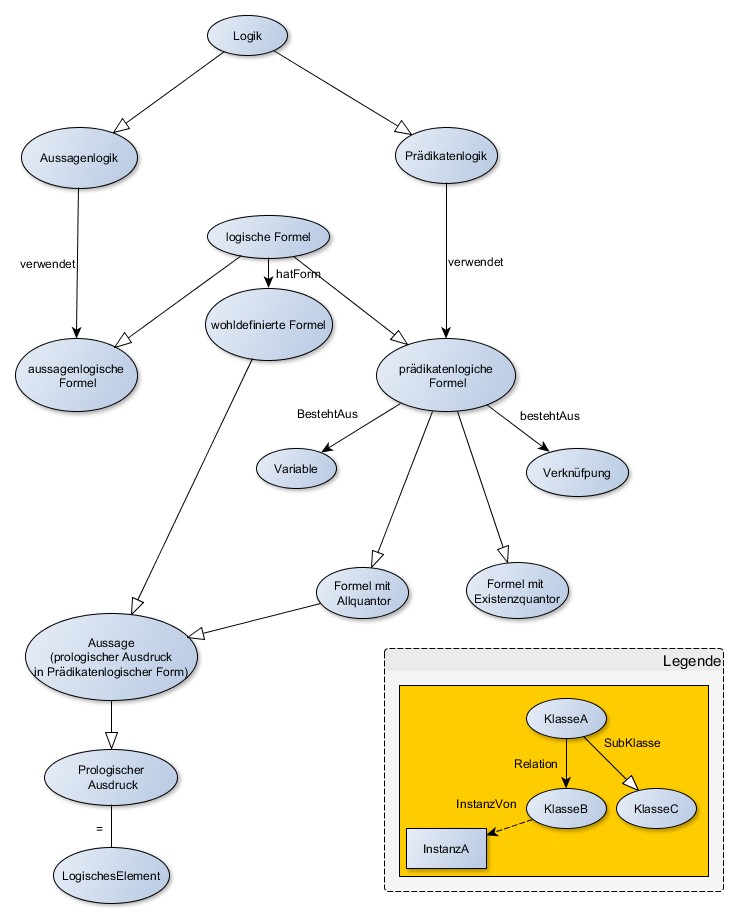
\includegraphics{bilder/formel_baum.png}}}
\caption{Vereinfachte Darstellung von Logik, rein mittels Klassen.\label{fig:prolog_logik_baum}\protect\footnotemark}
\end{figure}
\footnotetext{Eigene Darstellung mittels yEd.}

\newpage

Um auch Relationen abbilden zu können, wurde die Modellierung schliesslich mit Individuen erweitert. Dies erlaubte die Definition von Relationen zwischen diesen, was sich als Schritt in die richtige Richtung erweisen sollte.

\begin{figure}[H]
\centering \rotatebox{0}{\scalebox{0.3}[0.3]{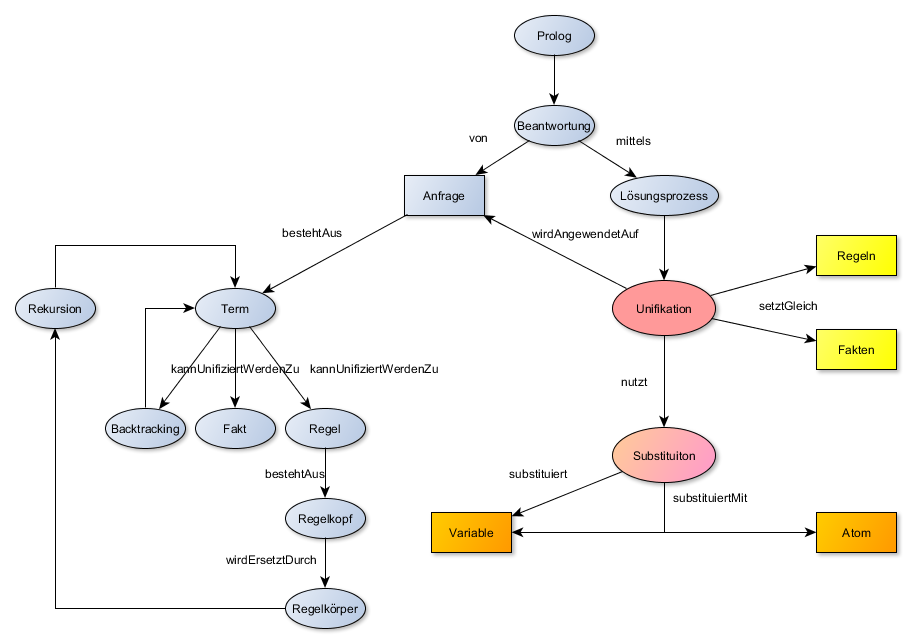
\includegraphics{bilder/loesungsprozess_baum.png}}}
\caption{Vereinfachte Darstellung eines Teils des Lösungsprozesses von Prolog, mittels Klassen, Individuen und Relationen.\label{fig:prolog_loesungsprozess}\protect\footnotemark}
\end{figure}
\footnotetext{Eigene Darstellung mittels yEd.}

Es wurde dann jeweils versucht konkrete Fragen aufgrund der erstellten Ontologie zu beantworten, wodurch Mängel in der Modellierung der Ontologie relativ gut sichtbar wurden. Diese zeigten sich zum Beispiel in Form von sehr umständlichen Abfragen um einfache Fakten abzufragen. Dies konnten dann schrittweise korrigiert werden, so dass die gewünschten Abfragen doch umgesetzt werden konnten. Details zu den gemachten Abfragen finden sich unter~\autoref{sec:anhang:sparql_beispiele}.

\begin{figure}[H]
\centering \rotatebox{0}{\scalebox{0.6}[0.6]{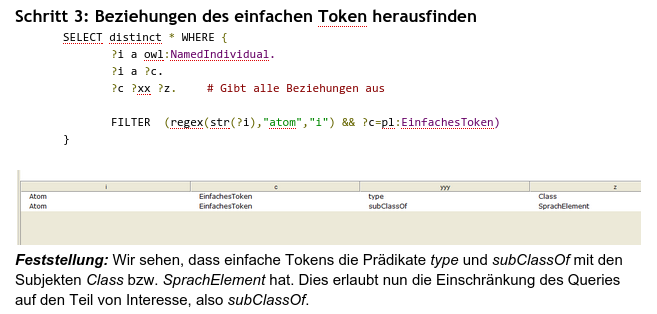
\includegraphics{bilder/sparql_beispiel.png}}}
\caption{Beispiel einer Abfrage der Ontologie mittels SPARQL.\label{fig:sparql_beispiel}\protect\footnotemark}
\end{figure}
\footnotetext{Eigene Darstellung mittels Stanford Protégé und Google Docs.}

Bei den genannten Mängeln handelte es sich nicht immer um solche, sondern es war schwierig abzugrenzen bei welchem Detaillierungsgrad die Modellierung aufhören soll. Es stellte sich also die Frage bei welcher Erklärungsgranulität aufgehört werden soll. So wurde schliesslich klar, dass eine zu feine Granularität solch einer Modellierung ins Uferlose gehen kann. Doch dies war nicht das Ziel, das Ziel war ein System zu schaffen und damit Erfahrungen zu gewinnen. Daraufhin empfahl der Betreuer der Arbeit, Herr Dr.\ Eckerle, Literatur über Prolog als Grundlage bzw.\ Rahmen zu verwenden. Hierbei wurde auf das Buch \textit{Künstliche Intelligenz} von \textit{U. Lämmel} und \textit{J. Cleeve} zurückgegriffen~\cite{laemmel}. Herr Dr.\ Eckerle empfahl sich dabei nur auf die Programmiersprache und deren Kernkonzepte zu beschränken, so wie sie auch im Buch beschrieben werden. Daraus resultierte eine verbesserte Modellierung der Ontologie von Prolog, mit Klassen, Relationen und Individuen.

\begin{figure}[H]
\centering \rotatebox{0}{\scalebox{0.15}[0.15]{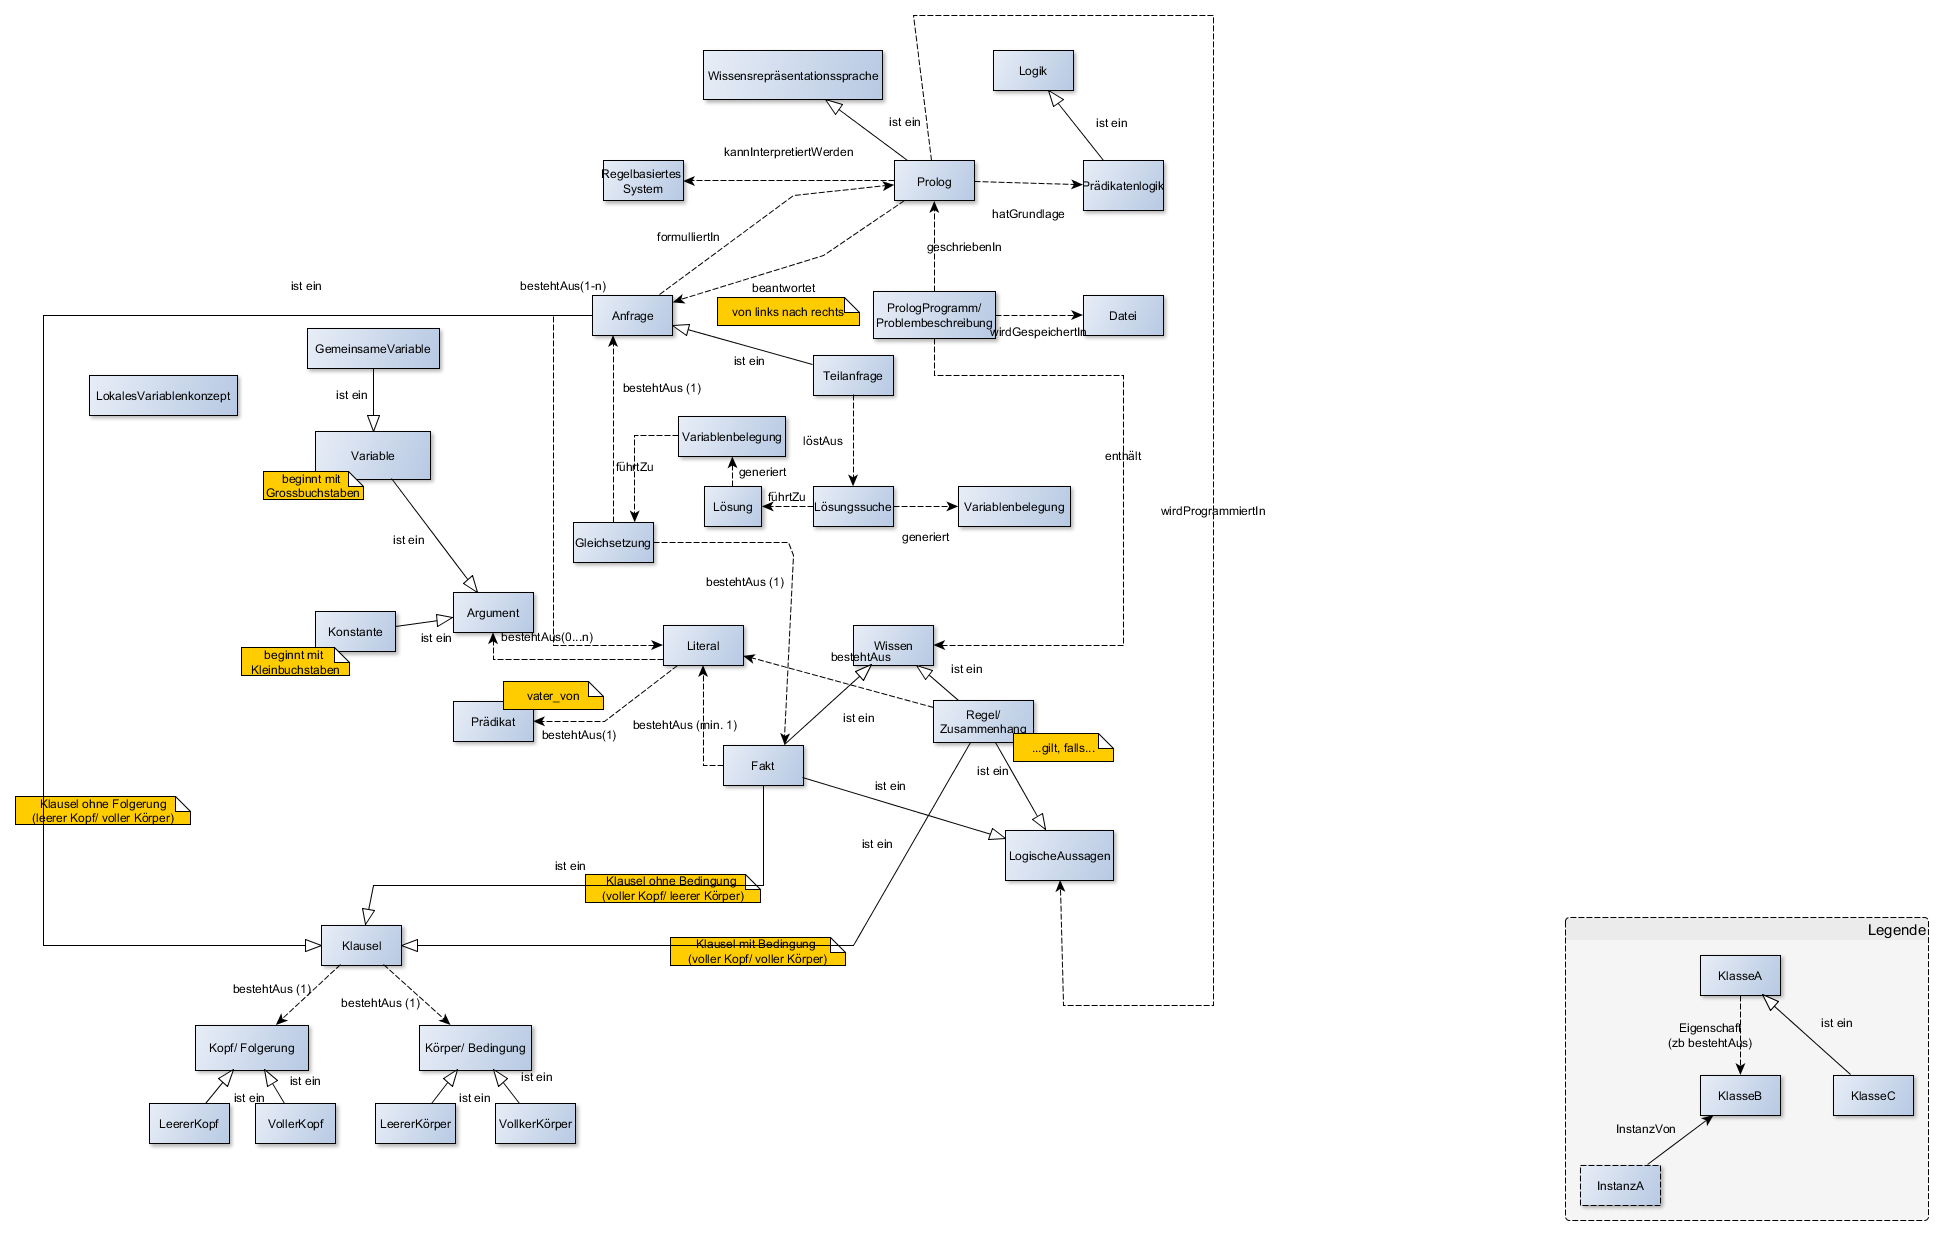
\includegraphics{bilder/prolog_baum.png}}}
\caption{Vereinfachte Darstellung von Prolog, mit Klassen und Relationen (Individuen wurden der Übersicht halber bewusst weggelassen).\label{fig:prolog_baum}\protect\footnotemark}
\end{figure}
\footnotetext{Eigene Darstellung mittels yEd.}

Dies erlaubte jedoch nach wie vor keinen zusätzlichen Gewinn von Mehrwert in Form von Inferenz. Nach diversen Gesprächen mit Herrn Dr.\ Eckerle, stellte sich heraus, dass der Ontologie Regeln fehlen. Es wurde dann versucht mithilfe von Prolog das Konzept von Prolog abzubilden. Die Idee dahinter war, von der objektorientierten Denkweise loszukommen. Für die Autoren war es einfach nachzuvollziehen, dass und wie in Prolog Regeln verwendet werden. In Prolog wurde auch schnell deutlich, dass eine Abfrage auf Fakten (ohne Regeln) keinen Mehrwert bringt.

Nach diversen, erfolglosen Versuchen Regeln zu finden, wurde dies zuerst anhand einfacher Modelle versucht. So zum Beispiel anhand des klassischen Beispiels des Familienstammbaums. Mit diesem simplen Beispiel wurde der Mehrwert einer Wissensmodellierung sogleich erkannt.

\begin{figure}[H]
\centering \rotatebox{0}{\scalebox{0.15}[0.15]{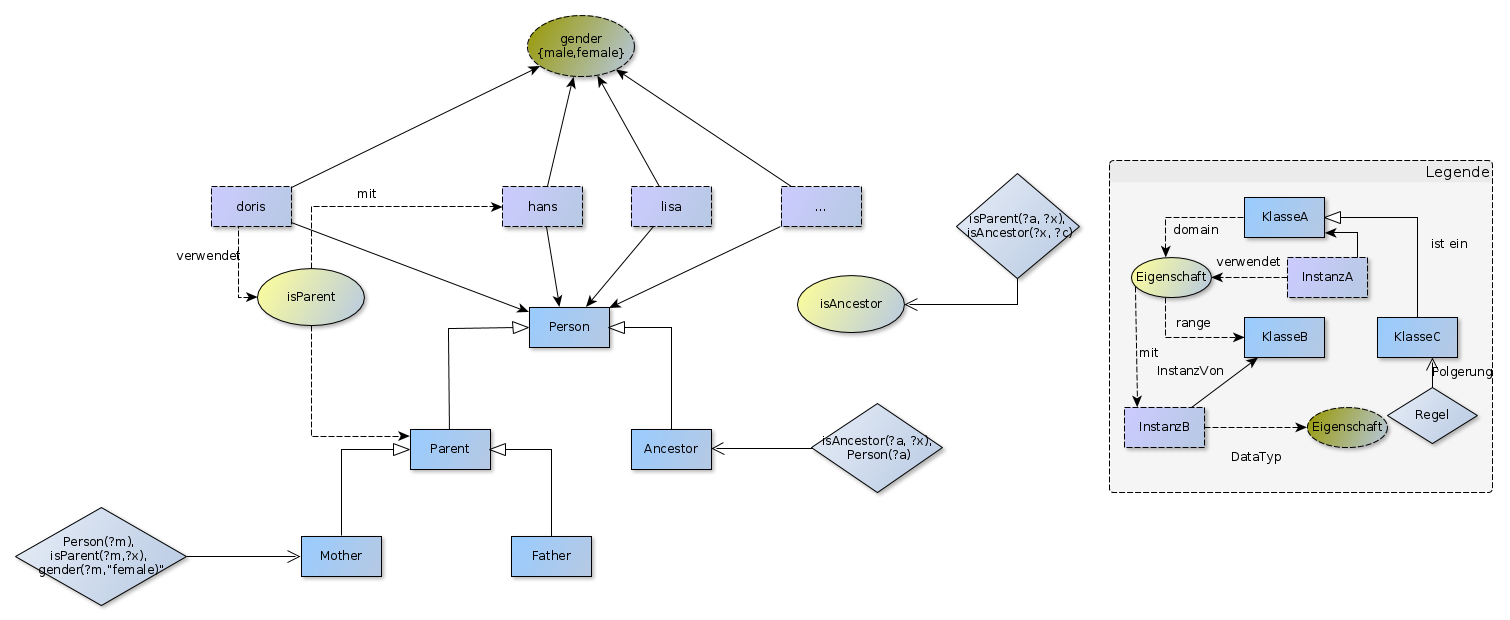
\includegraphics{bilder/familien_netz.png}}}
\caption{Darstellung eines einfachen Beispiels, der Abbildung einer Familie, mit Klassen, Individuen, Relationen und Regeln.\label{fig:familien_netz}\protect\footnotemark}
\end{figure}
\footnotetext{Eigene Darstellung mittels yEd.}

Jedoch gelang es auch nach dieser Erfahrung nicht, Regeln für die eigentliche Wissensdomäne zu finden. Die Erkenntnis aus diesem Prozess ist schlussendlich, dass die Abbildung von Prolog in einer Ontologie zwar möglich ist, jedoch eher in lexikalischer Form, was den Vorteil der Inferenz zunichtemacht. So kann beispielsweise gesagt werden, dass Prolog Unfikikation auf Anfragen anwendet und dabei Regeln mit Fakten gleichsetzt. Dabei wird Substitution genutzt, welche Variablen mit Variablen und/oder Atomen substituiert. Dies wurde aber Grösstenteils in Form von Fakten abgebildet. Einige wenige Regeln konnten erzeugt werden. Das damit abgebildete Wissen könnte aber auf eine einfachere und intuitivere Art mit Fakten abgebildet werden. Somit ist der Mehrwert der Regel nichtig. Die Regeln wurden dabei im Modul zur Erstellung von Regeln in der eingesetzten Anwendung zur Modellierung der Ontologie erfasst. Es handelt sich dabei um die Anwendung der Regelsprache SWRL, welche unter~\autoref{subsec:komponenten_protege_features} genauer beschrieben ist.

An dieser Stelle wurden  die Unterschiede der eingesetzten Anwendung zum Ziehen von Schlüssen (Pellet) bzw. der Mächtigkeit der Regeln gegenüber Prolog ersichtlich. Prolog ist hinsichtlich dieser Faktoren sehr flexibel. So ist man bei der Definition von Regeln nicht eingeschränkt, wobei diese beliebig viele Fakten und Prädikate enthalten können.

Im Unterschied dazu muss bei der eingesetzten Regelsprache SWRL jedes verwendete Konzept --- Klasse, Individuum, Eigenschaft oder Beziehung --- zuvor definiert sein. Es wird also explizit zwischen den verschiedenen Typen unterschieden. Bei Prolog wird dies nur durch die Menge der Argumente bzw. die Argumente selbst definiert. 

%[TODO: Reasoner Constraint Satisfaction]


\begin{figure}[H]
\centering \rotatebox{0}{\scalebox{0.2}[0.2]{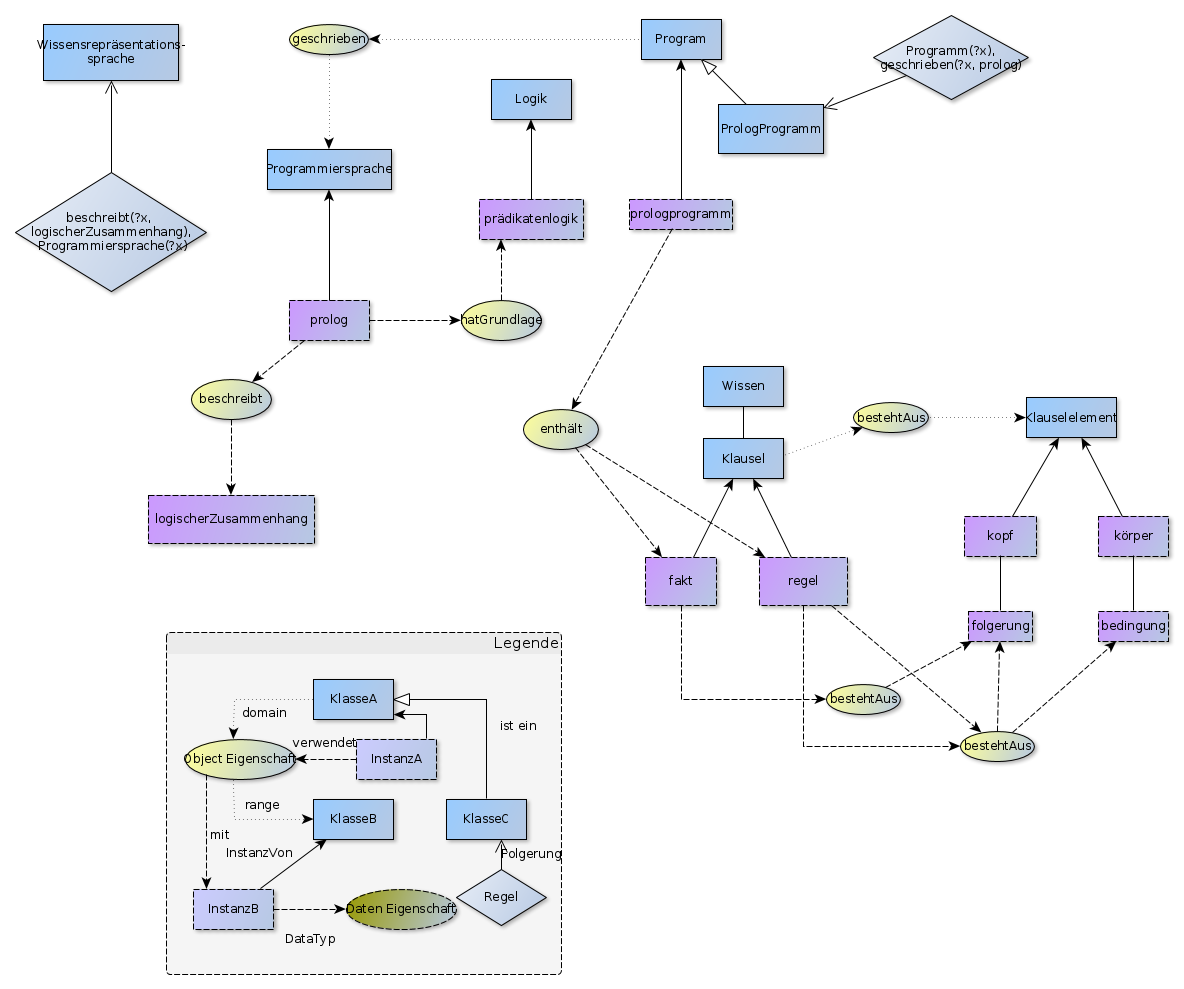
\includegraphics{bilder/prolog_netz.png}}}
\caption{Darstellung eines semantischen Netzes zur Abbildung von Prolog, mit Klassen, Individuen, Relationen und Regeln.\label{fig:prolog_netz}\protect\footnotemark}
\end{figure}
\footnotetext{Eigene Darstellung mittels yEd.}

Nach eingehender Analyse kamen die Autoren zum Schluss, dass sich die gewählte Domäne nicht eignet, um die Mächtigkeit einer Ontologie und dem damit verbundenen Reasoning abzubilden. Für die Wissensmodellierung bzw. Expertensysteme eignen sich also eher Wissensdomänen, welche Probleme mit konkreten Objekten abbilden. Im Gegensatz dazu befindet sich die ursprünglich gewählte Domäne auf einer zu hohen Abstraktionsebene. Daher ist dort der konkrete Nutzen, in Form von Inferenz, nicht direkt sichtbar.

Wie der Name Expertensystem schon andeutet, werden diese in Fällen verwendet, bei denen ein Fachexperte notwendig ist. Dieser kann mit seinem Fachwissen Schlüsse ziehen und so zusätzliches Wissen generieren.

Daher wurde eine andere Wissensdomäne --- die Planung von Reisen --- gewählt. Dies geht bereits eher in die Richtung von Expertensystemen, wofür semantische Netze am ehesten geeignet scheinen.

\subsubsection{Modellierung der tatsächlichen Ontologie}
\label{sub:modellierung_der_ontologie_tatsaechliche}

Nach dieser Entscheidung wurde mit der Modellierung also noch einmal beim Punkt null begonnen. Es konnte aber glücklicherweise auf den Erkenntnissen der vorigen Versuche aufgebaut werden.

Die Autoren entschieden sich anhand des gewonnen Wissens die Modellierung mittels konkreten Bespielen vorzunehmen. Basierend auf diesen wurde die Ontologie erzeugt und stetig erweitert. Zur Veranschaulichung ein konkretes Beispiel:

\begin{lstlisting}[caption={Konkretes Beispiel einer Reiseplanung.},captionpos=b]
    Familie Muster plant einen eintägige Ausflug. Die Kinder sind in einem Alter in dem Sie immer beschäftigt sein müssen.
\end{lstlisting}

\newpage

Dies ergab eine noch sehr simple Ontologie, welche mit diesem semantischen Netz abgebildet werden kann:

\begin{figure}[H]
\centering \rotatebox{0}{\scalebox{0.5}[0.5]{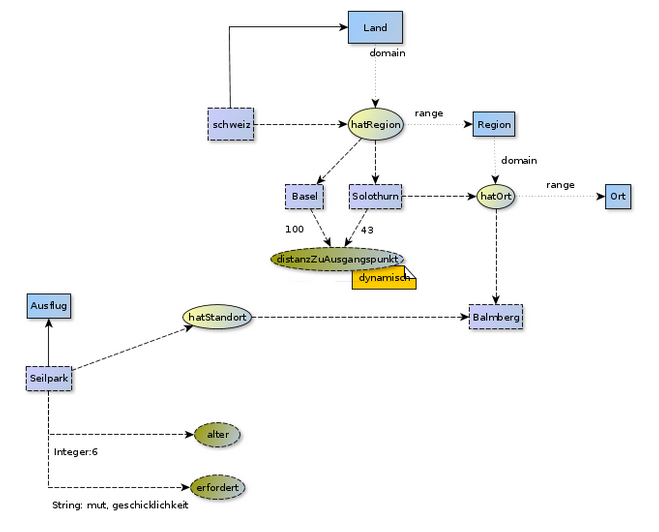
\includegraphics{bilder/famMuster.png}}}
\caption{Semantisches Netz für den Tagesausflug von Familie Muster.\label{fig:famMuster}\protect\footnotemark}
\end{figure}
\footnotetext{Eigene Darstellung mittels yEd.}

Mit der neu gewählten Wissensdomäne wurde auch der Sinn hinter der Verwendung von Regeln deutlich:
\begin{figure}[H]
    \centering \rotatebox{0}{\scalebox{0.5}[0.5]{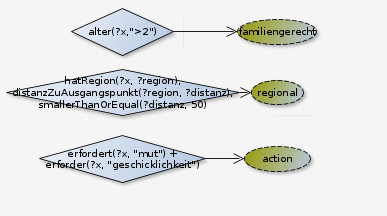
\includegraphics{bilder/famMusterRegeln.png}}}
    \caption{Regeln zum semantischen Netz für den Tagesausflug von Familie Muster.\label{fig:famMusterRegeln}\protect\footnotemark}
\end{figure}
\footnotetext{Eigene Darstellung mittels yEd.}

Aus der Modellierung konnten die folgenden Kriterien für die Abfrage abgeleitet werden:

\begin{itemize}
		\item familiengerecht
		\item action
		\item regional
\end{itemize}

Diese sind zugleich die Schlüsse der Regeln. Mit der richtigen SPARQL-Abfrage wird der Familie Muster schliesslich der Seilpark in Balmberg vorgeschlagen.

\begin{lstlisting}[caption={SPARQL-Abfrage um familiengerechte, regionale und actionreiche Ausflüge zu finden.},captionpos=b,language=SQL]
    SELECT
        *
    WHERE {
        ?object :familiengerecht true;
            :regional true;
            :action true.
        }
\end{lstlisting}


\begin{figure}[H]
\centering \rotatebox{0}{\scalebox{0.5}[0.5]{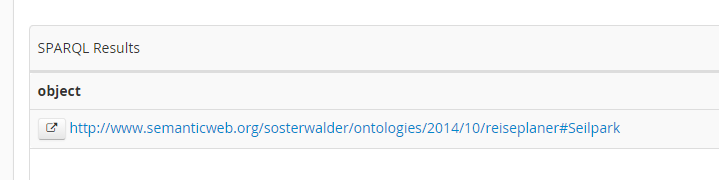
\includegraphics{bilder/famMusterOutput.png}}}
\caption{Ergebnis der Suche von Familie Muster.\label{fig:famMusterOutput}\protect\footnotemark}
\end{figure}
\footnotetext{Eigene Darstellung mittels yEd.}

In diesem ersten, bewusst sehr einfach gehaltenen Anwendungsfall, wird die Herangehensweise der Autoren sichtbar. Im Laufe von weiteren Beispielen wurde die Ontologie stetig erweitert. So haben die Autoren zum Beispiel erst zu einem späteren Zeitpunkt eine Zeiteinheit eingeführt oder gemerkt, dass die Eigenschaft familiengerecht zu oberflächlich und pauschal betrachtet wurde. Diese wurde dahingehend geändert, dass die Eigenschaft Untereigenschaften beinhaltet, welche unterscheiden in welchem Alter die Kinder sind. Die gesamte Ontologie wird im Kapitel {\color{red} TODO} genauer erläutert.

\subsection{Erstellung der Dokumentation zur Wissensmodellierung}
\label{subsec:dokumentation_wissensmodellierung}
Parallel zur Modellierung der Ontologie entstand eine Dokumentation des Vorgehens zur Wissensmodellierung. Diese zeigt exemplarisch auf, wie ein Knowledge-Engineer vorgeht, um eine Problemdomäne systematisch zu modellieren und formalisieren. Wie bereits zuvor erwähnt, wurde als Problemdomäne die Planung von Reisen gewählt. Die Dokumentation findet sich unter~\autoref{sec:anhang:tutorial_dokument}. -> In form eines Tutorials 

\subsubsection{Aufbau des Tutorials}
\label{subsec:dokumentation_wissensmodellierung_aufbau}
Im Gegensatz zu herkömmlichen Tutorials enthält das in dieser Arbeit erstellte einen grossen Theorieanteil. Aus diesem Grund wurde das Dokument in drei Aspekte aufgeteilt.

Da es sich hierbei um eine wissenschaftliche Arbeit handelt, haben die Autoren entschieden in einem erste Teil theoretischen Hintergrundwissen zur Wissensmodellierung bereitzustellen. So wird zum Beispiel erläutert, was Expertensysteme sind, wie diese graphisch dargestellt werden können und welche Schreibweisen respektive Sprachen verwendet werden um eine Ontologie abzubilden und darauf Abfragen zu stellen.

\noindent\rule[1ex]{\textwidth}{1pt}
\begin{wrapfigure}[4]{l}{0.1\textwidth}
    \vspace{-18pt}
    
\includegraphics[width=0.1\textwidth]{bilder/owl.png}
\end{wrapfigure}
Durch diese Eule wird die zweite Herangehensweise im Dokument eingeleitet. In diesem Teil liegt der Fokus auf praktischen Tipps der Autoren, auf Erfahrungen, welche gemacht wurden und welche mit Mehrwissen hätten vermieden werden können. Die Autoren versuchen dem Leser so die Arbeit zu vereinfachen.\\
\noindent\rule[1ex]{\textwidth}{1pt}

\noindent\rule[1ex]{\textwidth}{1pt}
\begin{wrapfigure}[4]{l}{0.1\textwidth}
    \vspace{-18pt}
    
\includegraphics[width=0.1\textwidth]{bilder/elephant.png}
\end{wrapfigure}
Der letzte Teil des Dokuments, welcher durch den Elefanten gekennzeichnet ist, verkörpert ein Tutorial im klassischen Sinne. Einem pragmatisch veranlagten Leser ist es so möglich, durch Folgen des Elefanten, innerhalb von kurzer Zeit ein simples Beispiel eines Expertensystems aufzubauen.\\
\noindent\rule[1ex]{\textwidth}{1pt}

\subsection{Erarbeitung der praktischen Grundlagen}
\label{subsec:praktische_grundlagen}

Die Erarbeitung der praktischen Grundlagen war die Vorarbeit für die Erstellung des Tutorial-Dokuments. Dementsprechend wurden die gewonnen Erkenntnisse darin eingearbeitet.

\subsection{Erstellung der abschliessenden Dokumentation}
\label{subsec:abschliessende_dokumentation}
Mit der Erstellung der abschliessenden Dokumentation ist das hier vorliegende Dokument gemeint.

TODO: ganzes vorgehen mit unseren verschiedenen Dokumenten  
